\section{Bonus question: a rule of radius 2}
\label{sec:bonus}

\subsection{The question}

The bonus question asks to \emph{use the implementation} to find a one-dimensional automaton
whose juxtaposed states draw a fractal or chaotic figure, with a rule that considers the two
cells to the left of the current cell and the two cells to its right. The figure must not be
obtainable with the left, current and right cells alone. There are $2^{2^5} = 2^{32}$ such rules,
about four billion.

\subsection{Method}

\paragraph{A fast simulator for a narrow problem.} The general engine evaluates a syntax tree
for every cell: it runs \emph{one} automaton of any dimension well, but trying thousands of rules
calls for something leaner. A two-state rule of radius 2 is entirely described by its truth
table, 32 output bits, hence a 32-bit number. \code{TableRule} stores that number and computes a
generation with one table lookup per cell, sliding a five-bit window along the row.

\paragraph{Families instead of four billion rules.} \code{RuleExplorer} explores three families:
the 64 \emph{totalistic} rules, whose result only depends on how many of the five cells are on,
exhaustively; and random samples of the $2^{20}$ left-right \emph{symmetric} rules or of all
rules. Rules that switch cells on in an empty row are skipped, since their whole background
flickers.

\paragraph{Measuring a picture.} Each rule is run for 255 generations from a single live cell,
on a row wide enough for the pattern never to reach the edges. The resulting picture is measured
in two ways.

\begin{itemize}
    \item The \emph{box-counting dimension}. Cover the picture with boxes of side $s$ and count
          those containing a live cell, $N(s)$. For a fractal, $N(s) \propto s^{-D}$; $D$ is estimated
          as the slope of the least-squares line through the points $(\log 1/s, \log N(s))$ for
          $s = 2, 4, \dots, 32$. A line has dimension 1, a filled area 2, and the Sierpi\'nski triangle
          $\log 3 / \log 2 \approx 1.585$.
    \item The \emph{compression ratio}. The cells are packed eight to a byte and deflated; the
          ratio of the compressed size to the packed size is close to 0 for uniform or periodic
          pictures, small for nested ones, and large for disordered ones.
\end{itemize}

The two numbers place a picture in one of four classes: \emph{extinct} (the last row is empty),
\emph{regular}, \emph{fractal} (dimension between 1.25 and 1.85) or \emph{chaotic} (dimension
above 1.85 and compression ratio above 0.30). The thresholds were calibrated on radius-1 rules
whose behavior is well known (\cref{tab:calibration}). The program measures $D = 1.585$ for rule
18, the theoretical value to three decimals, which validates the estimator.

\begin{table}[H]
    \centering\small
    \begin{tabular}{@{}lccl@{}}
        \toprule
        Radius-1 rule            & Dimension & Compression & Verdict \\
        \midrule
        4 (a lone cell persists) & 1.000     & 0.005       & regular \\
        254 (filled triangle)    & 1.962     & 0.057       & regular \\
        18 and 90 (Sierpi\'nski) & 1.585     & 0.061       & fractal \\
        150                      & 1.695     & 0.081       & fractal \\
        30                       & 1.944     & 0.386       & chaotic \\
        45                       & 1.988     & 0.587       & chaotic \\
        \bottomrule
    \end{tabular}
    \caption{Calibration of the classifier on elementary rules.}
    \label{tab:calibration}
\end{table}

This classification is a filter, not a proof: it shortlists candidates, and the final choice is
made by looking at the pictures.

\paragraph{Making sure radius 2 is needed.} A candidate is kept only if (1) its truth table
depends on at least one of the two outer cells, and (2) its picture differs from the picture of
\emph{each of the 256 rules of radius 1} run from the same row. The second test is what the
question literally asks.

\paragraph{Back to the general engine.} A rule worth keeping is translated into the rule
language: a totalistic rule becomes tests on \code{COMPTER} over the five cells, any other rule a
decision tree of \code{SI} operators over one-cell neighborhoods. The result is written as a
definition file and is, from then on, an automaton like any other. A test runs the fast simulator
and the general engine side by side on random radius-2 rules and checks that they agree on every
cell of every generation, so the two implementations validate each other.

\subsection{Results}

The command \code{cellula explore --write examples} explores the totalistic family in about a
second and reports 7 fractal and 6 chaotic rules that genuinely need radius 2. The best of each
kind (\cref{tab:bonus}, \cref{fig:bonus}) ships with the project as
\code{examples/radius2-fractal.xml} and \code{examples/radius2-chaotic.xml}.

\begin{table}[H]
    \centering\small
    \begin{tabularx}{\textwidth}{@{}l L L@{}}
        \toprule
                               & Fractal                                            & Chaotic          \\
        \midrule
        Rule, in words         & on when \emph{exactly one} of the five cells is on &
        on when \emph{one, two or four} of the five cells are on                                       \\
        Rule language          & \code{EQ(COMPTER(G4), 1)}                          &
        \code{OU(EQ(COMPTER(G4), 1), OU(EQ(COMPTER(G4), 2), EQ(COMPTER(G4), 4)))}                      \\
        Wolfram code           & 65\,814                                            & 1\,771\,542\,398 \\
        Box-counting dimension & 1.50                                               & 1.95             \\
        Compression ratio      & 0.03                                               & 0.43             \\
        \bottomrule
    \end{tabularx}
    \caption{The two rules retained, with
        $G4 = \{(-2), (-1), (0), (1), (2)\}$ declared in the files.}
    \label{tab:bonus}
\end{table}

\begin{figure}[H]
    \centering
    \begin{subfigure}[b]{\textwidth}
        \centering
        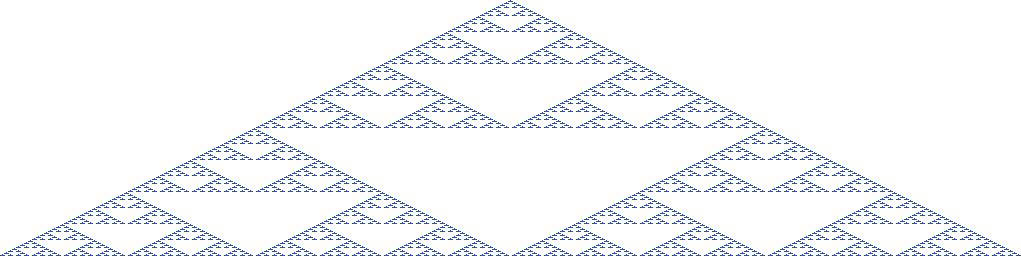
\includegraphics[width=0.92\textwidth]{radius2-fractal}
        \caption{Fractal: \code{EQ(COMPTER(G4), 1)}}
    \end{subfigure}\\[0.8em]
    \begin{subfigure}[b]{\textwidth}
        \centering
        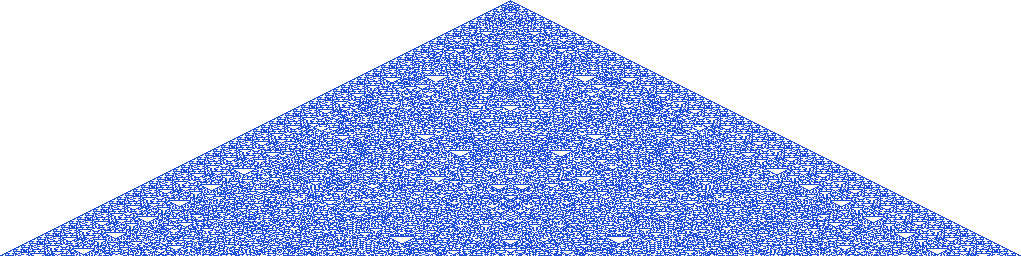
\includegraphics[width=0.92\textwidth]{radius2-chaotic}
        \caption{Chaotic: one, two or four live cells among the five}
    \end{subfigure}
    \caption{Generations 0 to 255 of the two radius-2 rules, from a single live cell, rendered by
        \code{cellula render}.}
    \label{fig:bonus}
\end{figure}

For these two rules there is also a one-line argument that no rule of radius 1 can draw the same
figure: their pattern widens by \emph{two} cells per generation on each side, whereas a rule of
radius 1 propagates information by at most one cell per generation.

Sampling 20\,000 rules of the symmetric or of the general family takes about eight seconds and
shortlists a few thousand candidates each; searches are reproducible thanks to a seed.
